\documentclass{standalone}
\usepackage{tikz}
\usepackage{ctex}
\setCJKmainfont{Noto Serif CJK SC}
\usepackage{mhchem,siunitx}
\usetikzlibrary{decorations.pathreplacing}
\begin{document}
\small
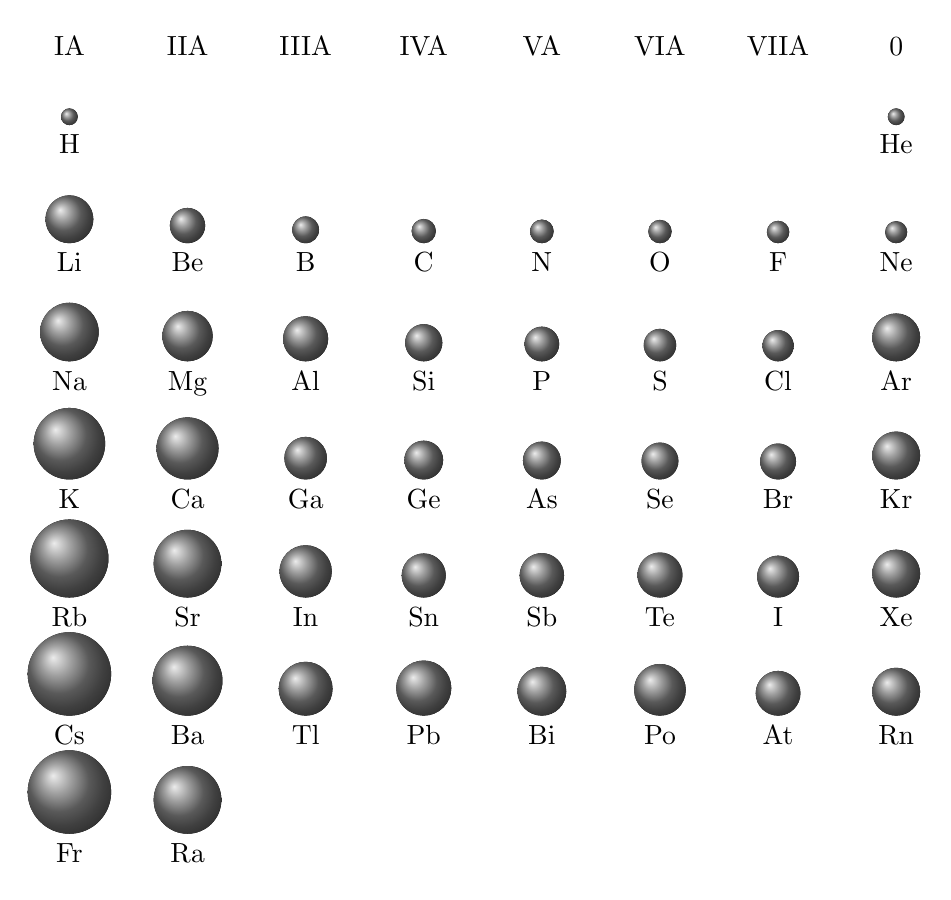
\begin{tikzpicture}
  \foreach \x[count=\i] in {IA,IIA,IIIA,IVA,VA,VIA,VIIA,0}
  {\node at (1.5*\i,0.5){\x};}
  \node at (1.5,-0.5)[below]{\ce{H}};
  \fill[ball color=gray](1.5,-0.394)circle(0.106);
  \node at (12,-0.5)[below]{\ce{He}};
  \fill[ball color=gray](12,-0.394)circle(0.106);
  \foreach \x/\y[count=\i] in {
    Li/1.52,
    Be/1.12,
    B/0.85,
    C/0.77,
    N/0.75,
    O/0.74,
    F/0.71,
    Ne/0.70%
  }
  {
    \node at (\i*1.5,-2)[below]{\ce{\x}};
    \fill[ball color=gray](\i*1.5,0.2*\y-2)circle(0.2*\y);
  }
  \foreach \x/\y[count=\i] in {
    Na/1.86,
    Mg/1.60,
    Al/1.43,
    Si/1.18,
    P/1.10,
    S/1.03,
    Cl/0.99,
    Ar/1.52%
  }
  {
    \node at (\i*1.5,-3.5)[below]{\ce{\x}};
    \fill[ball color=gray](\i*1.5,0.2*\y-3.5)circle(0.2*\y);
  }
  \foreach \x/\y[count=\i] in {
    K/2.27,
    Ca/1.97,
    Ga/1.35,
    Ge/1.23,
    As/1.20,
    Se/1.17,
    Br/1.14,
    Kr/1.52%
  }
  {
    \node at (\i*1.5,-5)[below]{\ce{\x}};
    \fill[ball color=gray](\i*1.5,0.2*\y-5)circle(0.2*\y);
  }
  \foreach \x/\y[count=\i] in {
    Rb/2.48,
    Sr/2.15,
    In/1.66,
    Sn/1.40,
    Sb/1.41,
    Te/1.43,
    I/1.33,
    Xe/1.52%
  }
  {
    \node at (\i*1.5,-6.5)[below]{\ce{\x}};
    \fill[ball color=gray](\i*1.5,0.2*\y-6.5)circle(0.2*\y);
  }
  \foreach \x/\y[count=\i] in {
    Cs/2.65,
    Ba/2.22,
    Tl/1.71,
    Pb/1.75,
    Bi/1.55,
    Po/1.64,
    At/1.42,
    Rn/1.52%
  }
  {
    \node at (\i*1.5,-8)[below]{\ce{\x}};
    \fill[ball color=gray](\i*1.5,0.2*\y-8)circle(0.2*\y);
  }
  \foreach \x/\y[count=\i] in {
    Fr/2.65,
    Ra/2.15%
  }
  {
    \node at (\i*1.5,-9.5)[below]{\ce{\x}};
    \fill[ball color=gray](\i*1.5,0.2*\y-9.5)circle(0.2*\y);
  }
\end{tikzpicture}
\end{document}